
\documentclass[12pt, a4paper]{article}

%-----------USEPACKAGE----------------------------
\usepackage{bm} % Tucne pismo
\usepackage[czech]{babel} % Cestina
\usepackage[T1]{fontenc}
\usepackage[utf8x]{inputenc}
\linespread{1.10} % Radkovani 1.3 odpovida radkovani 2
\usepackage{lmodern} % Daji se pouzit \HUGE atd.
\usepackage{amsmath}
\usepackage{algorithm}
\usepackage[noend]{algpseudocode} % Vkladani pseudo kodu
\usepackage{listings}
\usepackage{setspace}

% Graphics
\usepackage{graphicx}
\usepackage{epstopdf}
\usepackage{color}
\graphicspath{{./img/}}

% Hyperref and its color
\usepackage[unicode]{hyperref} % Odkazy v pdf, www a na e-mail
\usepackage[hypcap=true]{caption}
\usepackage[hypcap=true,list=true]{subcaption}
\hypersetup{colorlinks = true, citecolor = black}
\hypersetup{linkcolor=red}
\hypersetup{colorlinks,urlcolor=black}




%-----------COLORS--------------------------------
\definecolor{Code}{rgb}{0,0,0}
\definecolor{Decorators}{rgb}{0.5,0.5,0.5}
\definecolor{Numbers}{rgb}{0.5,0,0}
\definecolor{MatchingBrackets}{rgb}{0.25,0.5,0.5}
\definecolor{Keywords}{rgb}{0,0,1}
\definecolor{self}{rgb}{0,0,0}
\definecolor{Strings}{rgb}{0,0.63,0}
\definecolor{Comments}{rgb}{0,0.63,1}
\definecolor{Backquotes}{rgb}{0,0,0}
\definecolor{Classname}{rgb}{0,0,0}
\definecolor{FunctionName}{rgb}{0,0,0}
\definecolor{Operators}{rgb}{0,0,0}
\definecolor{Background}{rgb}{1, 1, 1}

%-----------LISTINGS-SETTINGS----------------------
\lstset{
	numbers=left,
	numberstyle=\footnotesize,
	numbersep=0.5em,
	xleftmargin=1.5em,
	xrightmargin=0em,
	framextopmargin=0em,
	framexbottommargin=0em,
	showspaces=false,
	showtabs=false,
	showstringspaces=false,
	frame=lrtb,
	tabsize=4,
	% Basic
	basicstyle=\ttfamily\footnotesize\setstretch{1},
	backgroundcolor=\color{Background},
	language=Python,
	% Comments
	commentstyle=\color{Comments}\slshape,
	% Strings
	stringstyle=\color{Strings},
	morecomment=[s][\color{Strings}]{"""}{"""},
	morecomment=[s][\color{Strings}]{'''}{'''},
	% Keywords
morekeywords={import,from,class,def,for,while,if,is,in,elif,else,not,and,or,print,break,continue,return,True,False,None,access,as,del,except,exec,finally,global,import,lambda,pass,print,raise,try,assert},
	keywordstyle={\color{Keywords}\bfseries},
	% Additional keywords
	morekeywords={[2]@invariant},
	keywordstyle={[2]\color{Decorators}\slshape},
	emph={self},
	emphstyle={\color{self}\slshape},
	breaklines=true, % Zalamuje radky.
}







%------------------VARIABLES----------------------------
\newcommand{\cisloCviceni}{2. cvičení}









%------------------LAYOUT----------------------------
\usepackage[top = 2.5 cm, bottom = 2.5 cm, left = 2.5 cm, right = 2.5 cm]{geometry} % geometrie stranky
\usepackage{longtable}% Pro dlouhy obsah, da se zalomit \pagebrek
\usepackage{fancyhdr}
\pagestyle{fancy}% Deffaultni nastaveni hlavicky a paticky
\setlength{\headheight}{16 pt}% Zvetsi hlavicku, aby to nedelalo warningy
\fancyhf{}
\lhead{\href{http://www.kky.zcu.cz/cs/courses/mpv}{Metody Počítačového Vidění}}
\rhead{\cisloCviceni}
\fancyfoot[R]{\thepage}
\fancyfoot[L]{Verze 2.0.0, poslední úpravy: \today}








%---------------BEGIN-DOCUMENT--------------------------
\begin{document}
 









 
%--------TITLE-PAGE--------------------------------------------
\begin{titlepage}
\begin{center}
	
\includegraphics[trim = 0.6cm 0.5cm 0.9cm 0.5cm, scale=1]{./FAV_logo_cz.pdf}
	\hspace*{\fill}
	
\includegraphics[trim = 3.5cm 1.5cm 2.6cm 2cm, scale=0.295]{./KKY_logo_cz.pdf}\\
	\vspace*{\fill}
	\textbf{\Huge{\href{http://www.kky.zcu.cz/cs/courses/mpv}{Metody Počítačového Vidění} \\ ~ \\ \cisloCviceni}}\\
	\vspace*{\fill}
	\textbf{\large{\href{mailto:LBures@kky.zcu.cz}{Ing. Lukáš Bureš}}} \hfill \textbf{\large{Plzeň, \today}}
\end{center}
\end{titlepage}












%--------OBSAH-CVICENI---------------------------------
\section*{Obsah cvičení}
\begin{enumerate}
	\item Graph Cut
	\item Popis Mean Shift shlukovacího algoritmu
	\item Výsledky Mean Shift algoritmu na 2D datech
\end{enumerate}



%--------MEAN-SHIFT-------------------------------
\section{Graph Cut}
\par{Algoritmus je uplatňován v oblasti počítačového vidění a může být efektivně použit na řadu low-level problémů, jako například vyhlazování obrazu, stereo korespondence, segmentace a mnoho dalších problémů, které mohou být formulovány s ohledem na minimalizaci energie.}

\par{\uv{Binární problémy} například segmentace je možné řešit pomocí tohoto algoritmu, avšak problémy, kde je možné pixely označit více štítky (hledání stereo korespondence, odstranění šumu v šedotónovém obrázku) nelze řešit přesně, ale řešení obvykle leží blízko globálního optima.}

\par{Pro segmentaci obrázku se používá metoda \href{http://en.wikipedia.org/wiki/GrabCut}{GrabCut}. Ukázku aplikace pro segmentaci obrazu v OpenCV je možné nalézt pod názvem \textit{grabcut.py} a metoda pro výpočet segmentace v OpenCV \href{http://docs.opencv.org/modules/imgproc/doc/miscellaneous_transformations.html?highlight=grabcut#cv2.grabCut}{\textit{grabCut}}.}

\begin{figure}[!ht]
	\centering
	\begin{minipage}[t]{0.5\textwidth}
		%trim option's parameter order: left bottom right top
		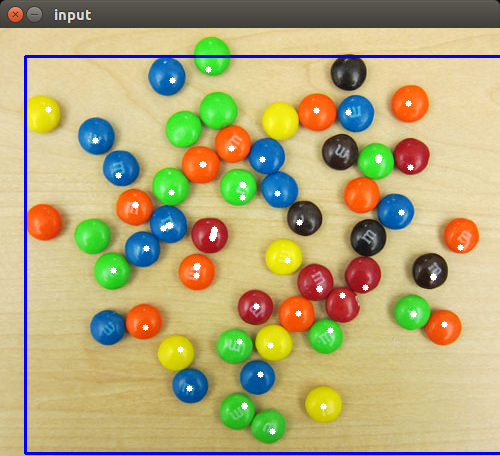
\includegraphics[width = \textwidth]{grabcut_input.png}
	\caption{Vstupní obrázek s oknem, ve kterém má být algoritmus aplikován společně s~informací od učitele (označené popředí).}
		\label{fig:grabcut_input}
	\end{minipage}%
	\hfill
	\begin{minipage}[t]{0.5\textwidth}
		%trim option's parameter order: left bottom right top
		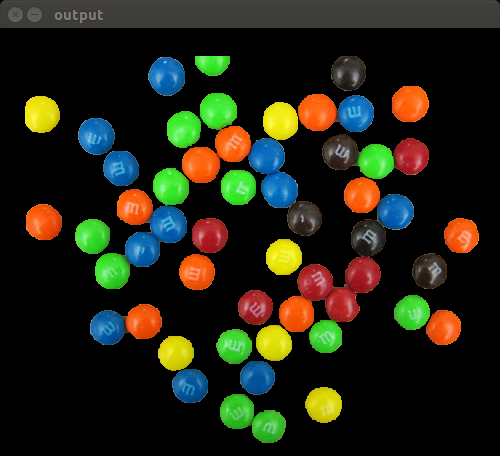
\includegraphics[width = \textwidth]{grabcut_output.png}
		\caption{Výsledná segmentace.}
		\label{fig:grabcut_output}
	\end{minipage}%
\end{figure}

\par{Ukázka vyžaduje na vstup ohraničující rámeček plus volitelně informaci o tom, které pixely patří do pozadí (vše co nechceme segmentovat), a které do popředí (objekty).}

\newpage











%--------MEAN-SHIFT-------------------------------
\section{Popis Mean Shift shlukovacího algoritmu}
\begin{algorithm}[!ht]
	\caption{Mean Shift algoritmus.}
	\label{alg:MeanShift2D}
	\begin{algorithmic}[1]
		\State Vstup: Vstupní data $\bm{x} \in X$ a poloměr okénka $r$ (průměr okénka $d = 2r + 1$).
		\State Inicializace: počet shluků $i = 1$, tedy $\exists S_1$.
		\While{$\exists \bm{x}$, který nemá žádný hlas o přiřazení do shluku $S_i$}
			\State Zvolí náhodně startovací střed $\bm{c}_1 \in X$, který nemá žádný hlas o přiřazení do shluku.
			\While{$\bm{c}_j \neq \bm{c}_{j+1}$}
				\State Vypočti vzdálenost $\forall \bm{x}$ od aktuálního středu $\bm{c}_j$, $distance = \| \bm{c}_j - \bm{x} \|$.
				\State $\forall \bm{x}$, pro které platí $distance < r$ vypočti vážený průměr a nastav ho, jako střed $\bm{c}_{j+1}$ pro další iteraci $j+1$,
					\begin{equation}
						\bm{c}_{j+1}	= \frac{\sum_{l} \bm{x}_l w_l }{\sum_{k} w_k},
					\end{equation}
					kde $w$ jsou váhy (počet výskytů daného vzorku $\bm{x} \in X$). 
				\If{$\bm{c}_j == \bm{c}_{j+1}$}
					\If{$i == 1$}
						\State Ulož číslo $i$ vytvořeného shluku a jeho střed $\bm{c}_{j+1}$.
						\State Ulož hlas pro $\forall \bm{x}$, které byly cestou navštíveny.
					\Else
						\If{$\exists \bm{c}_{j+1} \in C$}
							\State Ulož hlas pro $\forall \bm{x}$, které byly cestou navštíveny. 
						\Else
							\State Vytvoř nový shluk $i + 1$ a ulož jeho střed $\bm{c}_{j+1}$. 							\State Ulož hlas pro $\forall \bm{x}$, které byly cestou navštíveny. 
						\EndIf
					\EndIf
				\EndIf
			\EndWhile			
		\EndWhile
		\State $\forall \bm{x} \in X$ nastav takový shluk, který má nejvíce hlasů.
	\end{algorithmic}
\end{algorithm}
\begin{figure}[!ht]
	\centering
	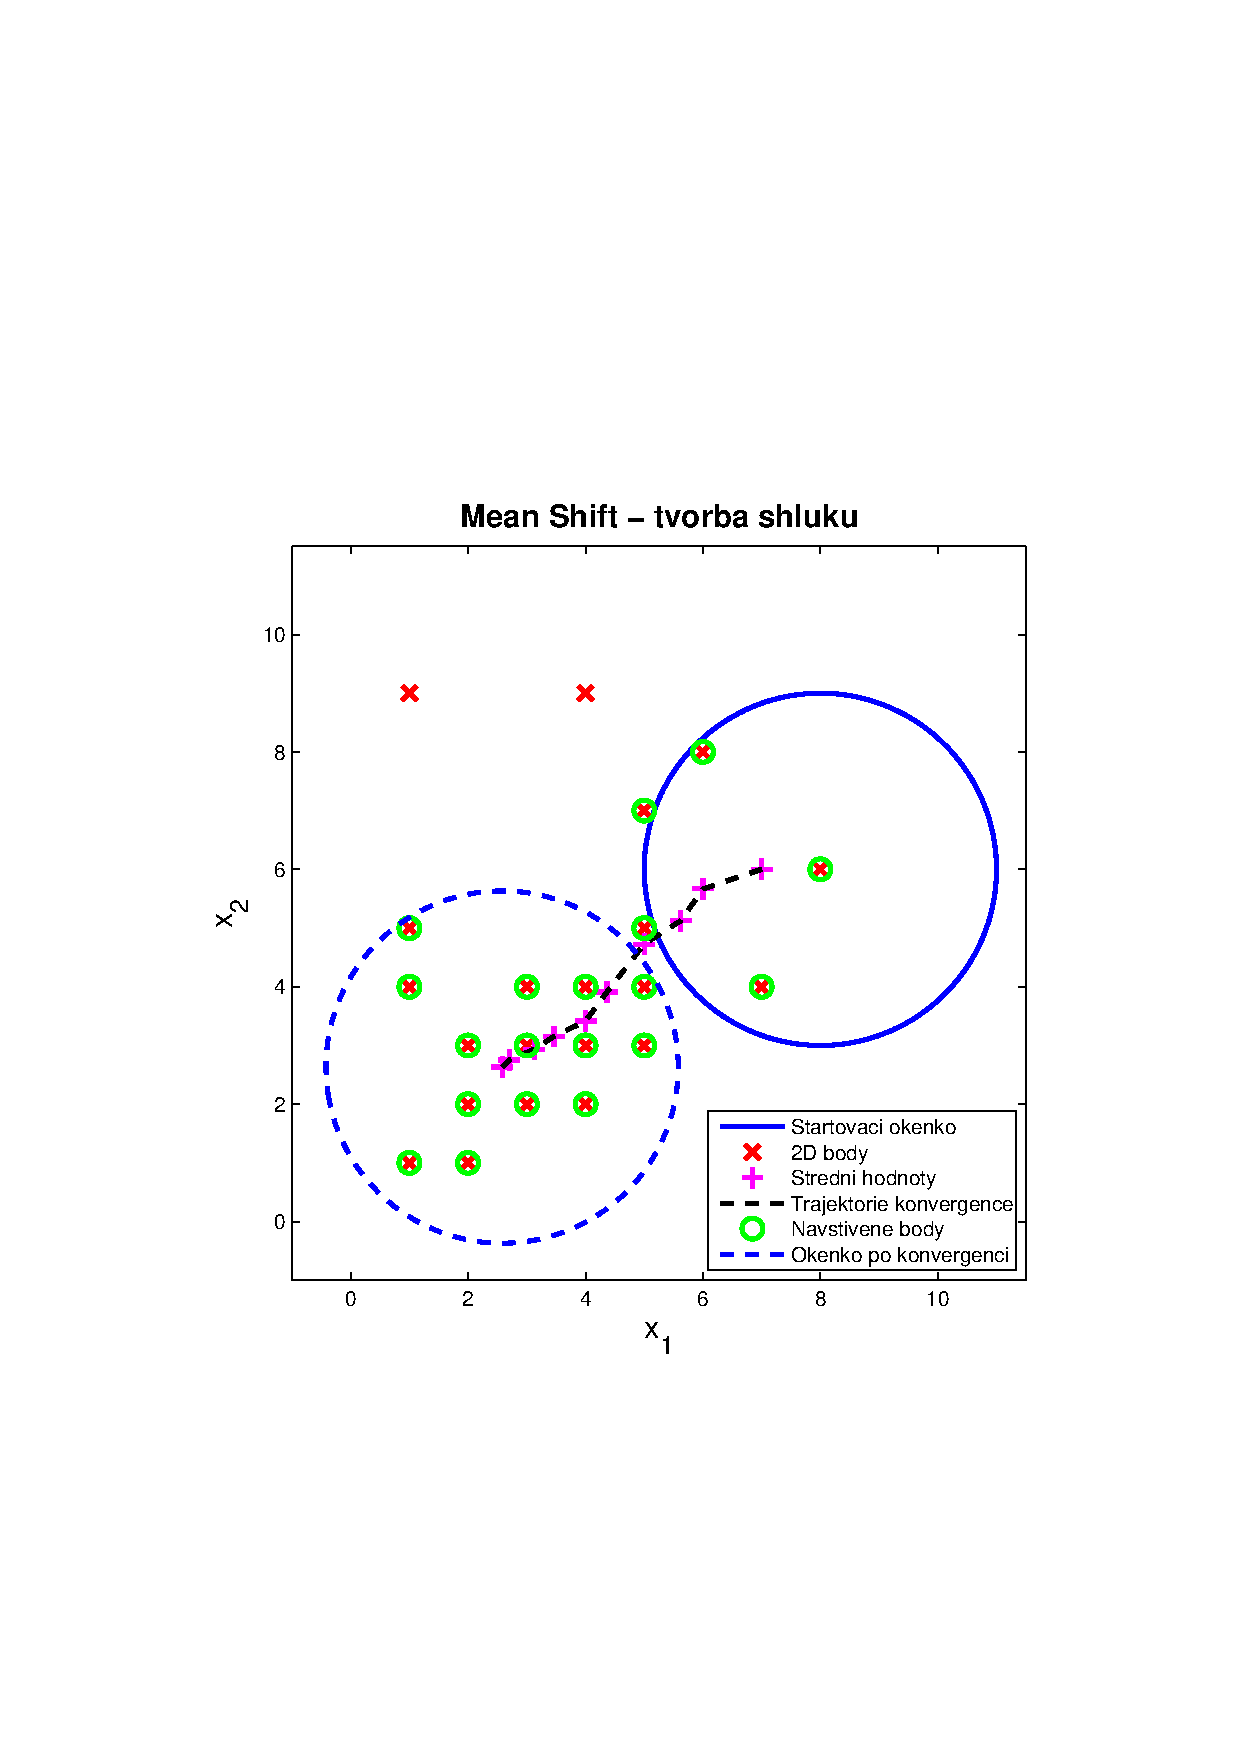
\includegraphics[width = 0.65\textwidth, trim = 3.5cm 8.5cm 3.5cm 9.5cm]{MeanShift.pdf}
	\label{fig:MeanShift}
\end{figure}

\newpage













%--------MEAN-SHIFT-------------------------------
\section{Výsledky Mean Shift algoritmu na 2D datech}
\par{Vstupní data pro naši 2D úlohu získáme následujícím postupem. Načtený barevný RGB obrázek převedeme do HSV formátu (Hue, Saturation, Value) a využijeme pouze hodnoty Hue pro $x$-ovou a Saturation pro $y$-ovou osu. Nad takto získanými daty provedeme Mean Shift algoritmus.}



\begin{figure}[!ht]
	\centering
	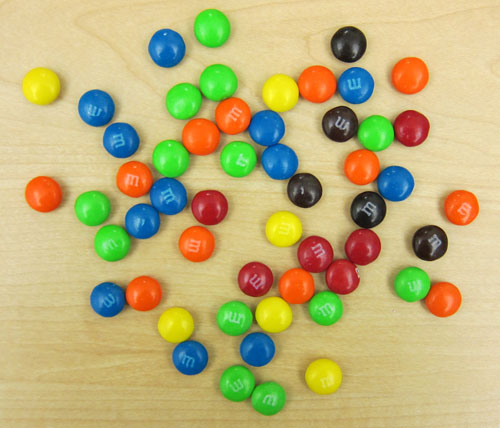
\includegraphics[width = 0.65\textwidth]{mms.jpg}
	\caption{Vstupní RGB obrázek.}	
	\label{fig:mms}
\end{figure}

\begin{figure}[!ht]
	\centering
	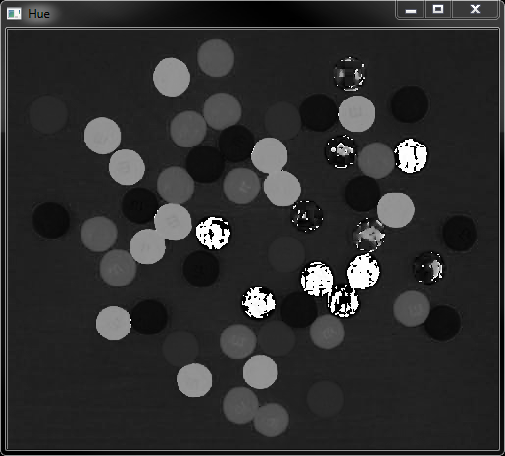
\includegraphics[width = 0.65\textwidth]{Hue.png}
	\caption{Obrázek \ref{fig:mms} převeden do formátu HSV a zobrazena Hue složka.}	
	\label{fig:Hue}
\end{figure}

\begin{figure}[!ht]
	\centering
	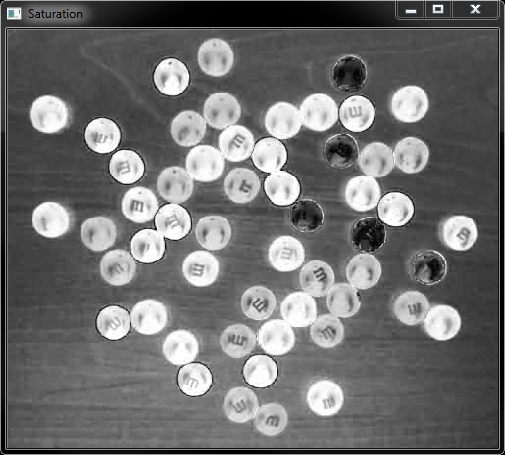
\includegraphics[width = 0.65\textwidth]{Saturation.png}
	\caption{Obrázek \ref{fig:mms} převeden do formátu HSV a zobrazena Saturation složka.}	
	\label{fig:Saturation}
\end{figure}

\begin{figure}[!ht]
	\centering
	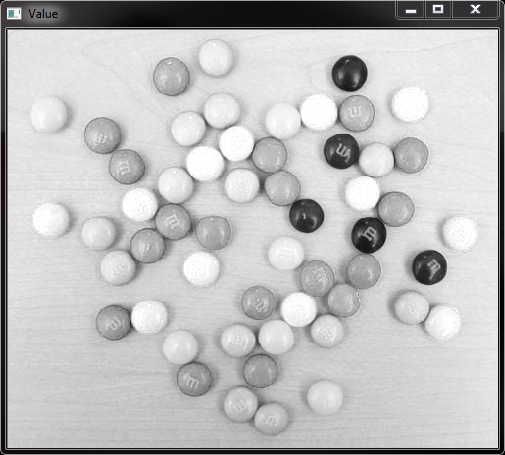
\includegraphics[width = 0.65\textwidth]{Value.png}
	\caption{Obrázek \ref{fig:mms} převeden do formátu HSV a zobrazena Value složka.}	
	\label{fig:Value}
\end{figure}

\begin{figure}[!ht]
	\centering
	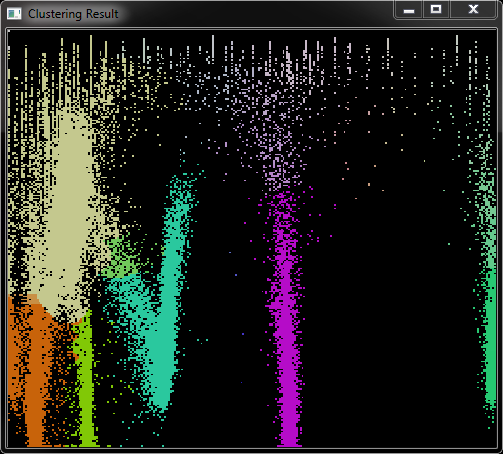
\includegraphics[width = 0.65\textwidth]{ClusteringResult.png}
	\caption{Výsledné shluky v HS prostoru.}	
	\label{fig:ClusteringResult}
\end{figure}

\begin{figure}[!ht]
	\centering
	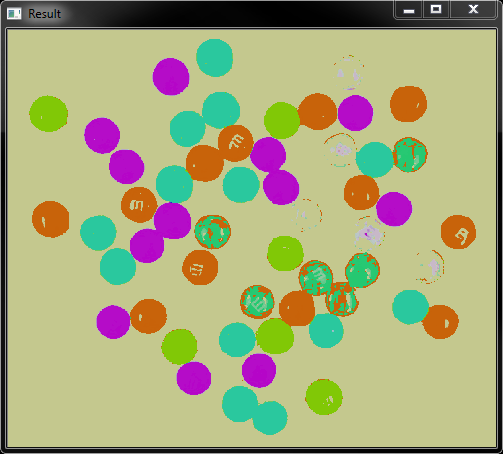
\includegraphics[width = 0.65\textwidth]{Result.png}
	\caption{Nahrazení HS hodnot středními hodnotami shluku (Value = 200).}	
	\label{fig:Result}
\end{figure}

\begin{figure}[!ht]
	\centering
	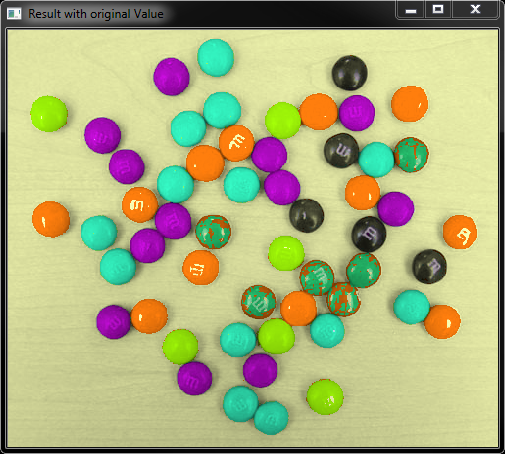
\includegraphics[width = 0.65\textwidth]{ResultWithOriginalValue.png}
	\caption{Nahrazení HS hodnot středními hodnotami shluku (Value = originální hodnoty).}	
	\label{fig:ResultWithOriginalValue}
\end{figure}

















\end{document}



















